\documentclass[a4paper,10pt]{article}
\usepackage[utf8]{inputenc}
\usepackage[spanish]{babel}
%links en el indice
\usepackage[bookmarks = true, colorlinks=true, linkcolor = black, citecolor = black, menucolor = black, urlcolor = black]{hyperref} 
\usepackage{graphicx}



%opening
\title{Triage, Sistema de gestión para sala de Guardia Hospitalaria}
\author{\textit{Manual del usuario}}

\newcommand{\mySection}[1]{\section{#1}}
\newcommand{\mySubSection}[1]{\subsection{#1}}

\begin{document}


\maketitle
\newpage 

\begin{abstract}
El presente documento tiene como objetivo describir y explicar las funcionalidades del Sistema de gestión para sala de Guardia Hospitalaria, que utiliza el método Triage para la recepción de los pacientes.

En el mismo, se detalla la funcionalidad de cada pantalla con screenshot y ejemplos básicos y funcionales al manual.

\end{abstract}


\newpage 
\tableofcontents

\newpage

\section{Manual del Usuario}
Las siguientes secciones tienen como objetivo describir y explicar las funcionalidades del Sistema de gestión para sala de Guardia Hospitalaria, que utiliza el método Triage para la recepción de los pacientes. En las mismas, se detalla la funcionalidad de cada pantalla con screenshot y ejemplos básicos y funcionales al manual.

Triage es un método de medicina de emergencias y desastres para la selección y clasificación de los pacientes basándose en las prioridades de atención. La guardia del H.Z.G.A ``Dr.\ Arturo Oñativia'' de la localidad de Rafael Calzada utiliza este sistema para clasificar a sus pacientes. El triage prioriza el compromiso vital inmediato y las posibles complicaciones.
Los pacientes pueden ser clasificados con tres Prioridades:

\begin{description}
\item[Prioridad 1] \mbox{} \\ 
Cuando el paciente tiene posibilidad de sobrevivir y la actuación médica debe ser inmediata.
\item[Prioridad 2] \mbox{} \\ 
Pacientes que presentan una situación de urgencia con riesgo vital.
\item[Prioridad 3] \mbox{} \\ 
Paciente levemente lesionado, que puede caminar y su traslado no precisa medio especial.

\end{description}



\mySection{Ingreso al sistema (\textit{login}) y cambio de contraseña}
En esta sección explicamos como ingresar al sistema y como cambiar la contraseña.

\mySubSection{Ingreso al sistema (\textit{login})}
La primer pantalla que vemos al ingresar a la aplicación es la de \textit{login} (figura \ref{fig:login}).
\begin{figure}[h]
\centerline{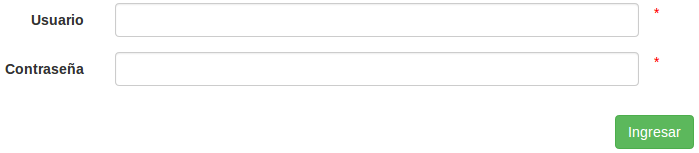
\includegraphics[width=0.7\textwidth]{login.png}}
\caption{Pantalla de ingreso al sistema}
\label{fig:login}
\end{figure}
Allí debemos ingresar correctamente el usuario y la contraseña. Si ingresamos mal alguno de los campos no podremos ingresar al sistema y se nos muestra un mensaje de error (figura \ref{fig:login_fallido}).
\begin{figure}
\centerline{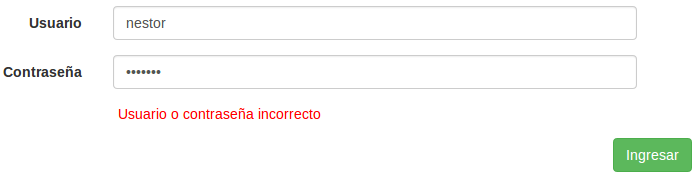
\includegraphics[width=0.7\textwidth]{login_fallido.png}}
\caption{Login fallido}
\label{fig:login_fallido}
\end{figure}

\mySubSection{Cambio de contraseña}\label{cap:cambio_pass}
Para acceder a la pantalla de cambio de contraseña nos dirigimos hacia el nombre del usuario actual y luego a ``Cambiar contraseña'' (ver figura \ref{fig:menu_cambio_pass}).
\begin{figure}
\centerline{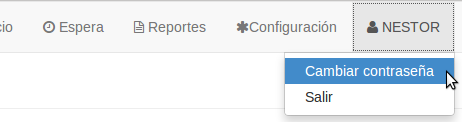
\includegraphics[width=0.7\textwidth]{menu_cambio_pass.png}}
\caption{Menú de cambio de contraseña}
\label{fig:menu_cambio_pass}
\end{figure}
Allí debemos ingresar la contraseña actual y la nueva (dos veces) (figura \ref{fig:cambio_pass}).
\begin{figure}
\centerline{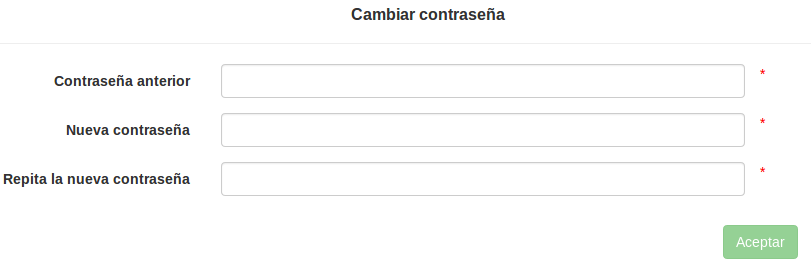
\includegraphics[width=0.7\textwidth]{cambio_pass.png}}
\caption{Cambio de contraseña}
\label{fig:cambio_pass}
\end{figure}
Validaciones a tener en cuenta:

\begin{itemize}
\item El nombre del usuario debe tener al menos tres caracteres.
\item La contraseña debe tener al menos 4 caracteres.
\item Para la contraseña el sistema distingue entre mayúsculas y minúsculas. Si, por ejemplo, nuestra contraseña es ``Clave'' y en la pantalla de \textit{login} ingresamos ``clave'', no podremos ingresar al sistema.
\item Siempre que se crea un usuario nuevo la contraseña por default es ``triage''.
\end{itemize}

\section{Pantalla Inicial}
En esta sección del manual explicaremos cómo ingresar nuevas personas al sistema o cómo buscarlas en el caso de que ya hayan sido atendidas.

\subsection{Ingreso de un nuevo paciente}
En la pantalla de Inicio del sistema (figura \ref{fig:inicio}) 
\begin{figure}
\centerline{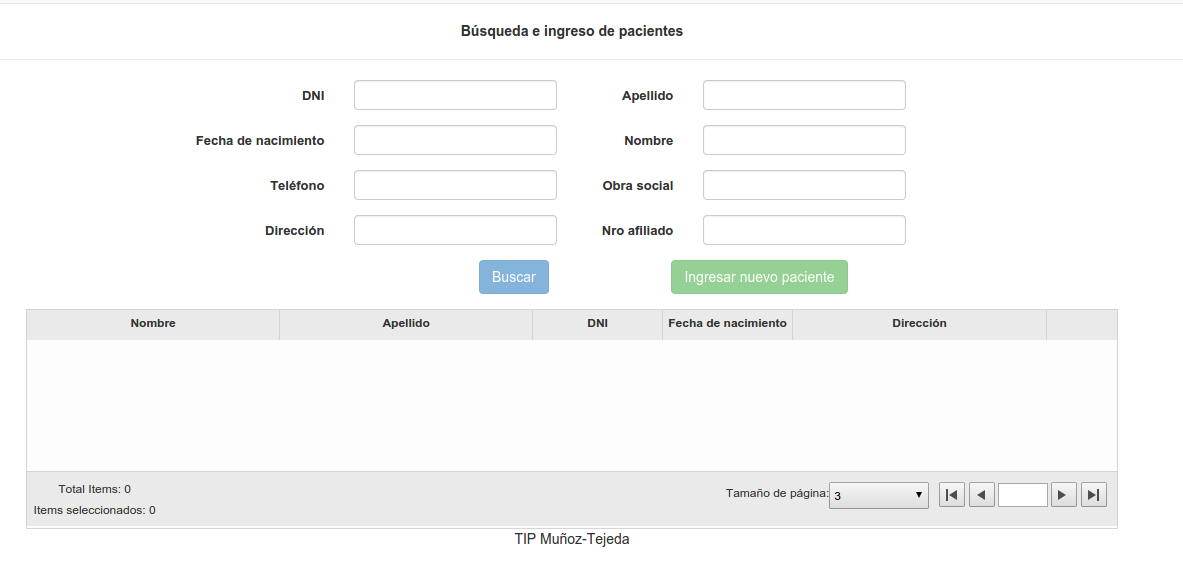
\includegraphics[width=0.99\textwidth]{inicio.png}}
\caption{Pantalla inicial} \label{fig:inicio}
\end{figure}
se pueden ver los campos identitificatorios de las personas. El botón ``Ingresar nuevo paciente'' aparecerá deshabilitado hasta completar los campos obligatorios: DNI, nombre, apellido y fecha de nacimiento (como puede verse en la figura \ref{fig:inicio_nuevo}).
\begin{figure}
\centerline{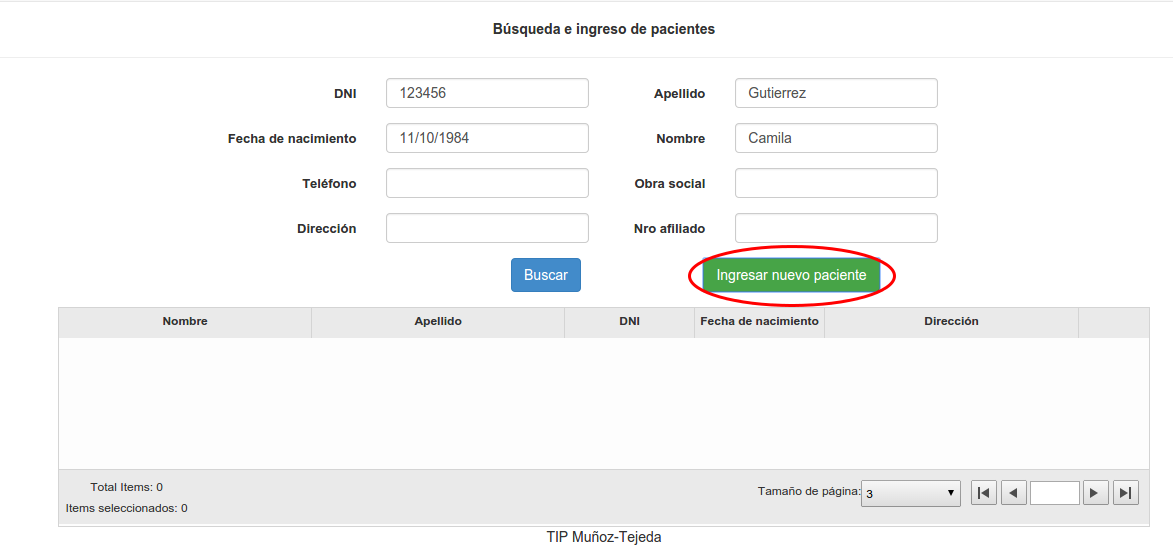
\includegraphics[width=0.99\textwidth]{inicio_nuevo.png}}
\caption{Botón habilitado para poder cargar nuevo paciente} \label{fig:inicio_nuevo}
\end{figure}
Al presionar dicho botón, el sistema guardará los datos de esa persona y redigirá la aplicación a la ventana de Triage para comenzar con la carga de síntomas.

\subsection{Búsqueda e ingreso de un paciente cargado en sistema}
En el caso de que el paciente ya haya recibido atención en la guardia, es posible buscarlo en la aplicación. El botón ``buscar'' apacerá deshabilitado hasta que se complete alguno de los campos (figura \ref{fig:inicio_busqueda}).
\begin{figure}
\centerline{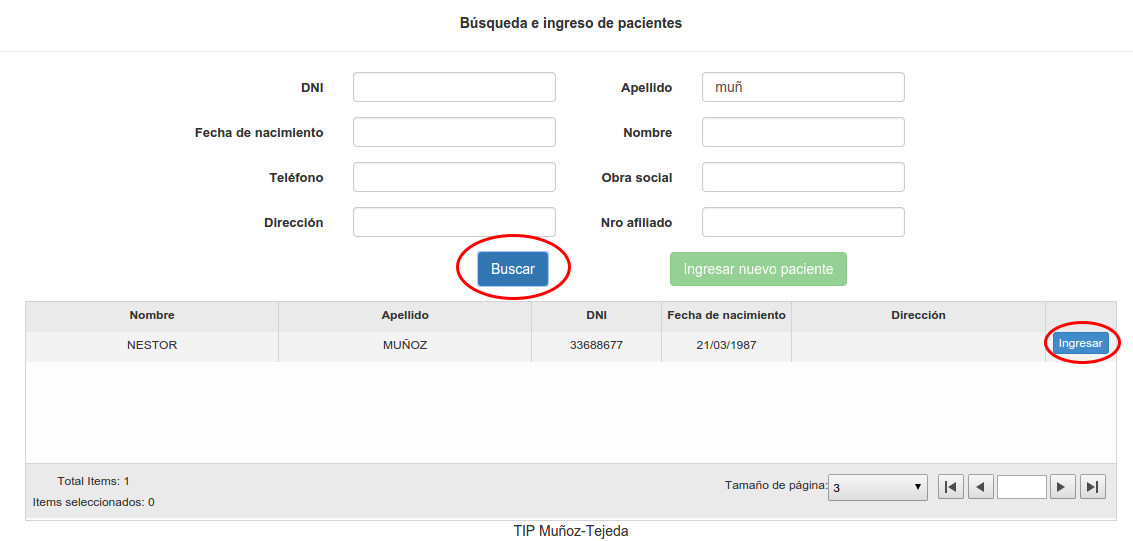
\includegraphics[width=0.99\textwidth]{inicio_busqueda.png}}
\caption{Botón habilitado para poder buscar un paciente y botón para ingresar al paciente a Triage} \label{fig:inicio_busqueda}
\end{figure}
Una vez presionado el botón para buscar, el sistema muestra en el listado inferior la lista de personas que coinciden con los criterios de búsqueda ingresados (ver sección \ref{cap:filtrado_listado}). En el caso de ver a la persona que se está buscando, en la lista aparece el botón ``Ingresar''. Al presionarlo, el sistema redirige la aplicación a la ventana de Triage para comenzar con la carga de síntomas.

\subsection{Filtrado de un listado}\label{cap:filtrado_listado}
Todos los listados de la aplicación pueden ser filtrados para facilitar la búsqueda de algún registro. El modo de filtrado es muy sencillo. Los pasos a seguir son los siguientes:
\begin{enumerate}
\item ingresamos algun texto en el/los campo/s de búsqueda (no hace falta que ingresemos la palabra entera de lo que buscamos, es suficiente si solo ingresamos las primeras letras)
\item presionamos el boton ``Buscar''
\end{enumerate}



\section{Triage}
En esta sección daremos a conocer el camino que recorre la aplicación para cargar los síntomas del paciente.

\subsection{Pantalla inicial de Triage}
La pantalla inicial de Triage (como podemos ver en la figura \ref{fig:triage_inicial}) 
\begin{figure}
\centerline{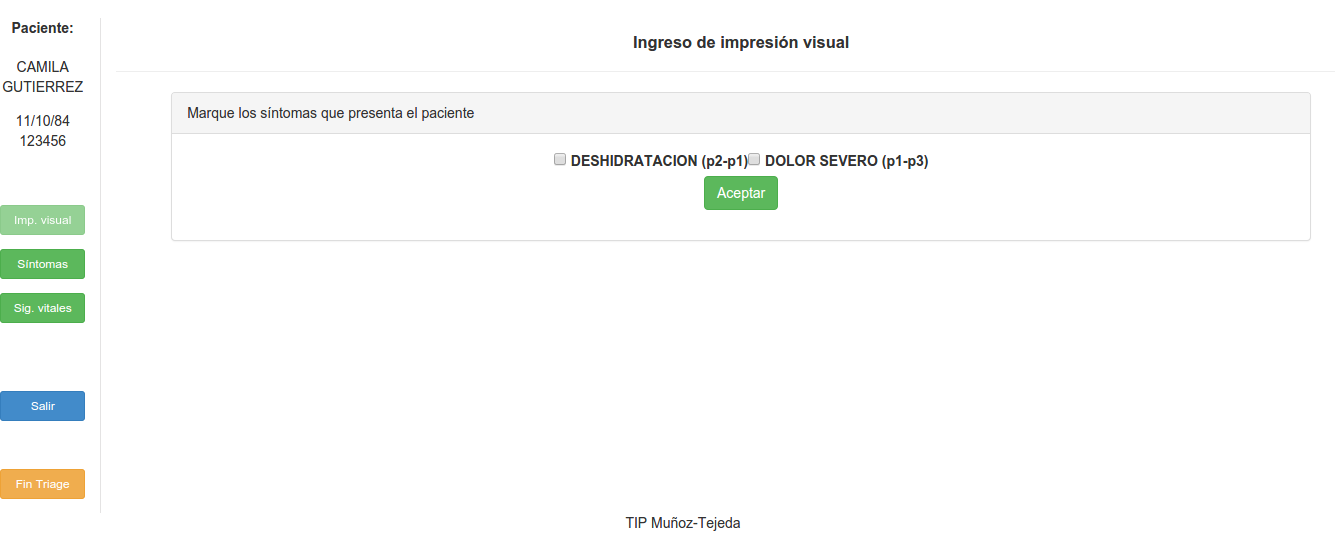
\includegraphics[width=0.99\textwidth]{impresion_visual.png}}
\caption{Pantalla inicial de Triage} \label{fig:triage_inicial}
\end{figure}
tiene una navegación definida por pestañas (que se pueden ver en la parte izquierda de la pantalla). Las pestañas permiten cambiar de pantalla de manera rápida y simple.

\subsection{Impresión Visual}
En la pestaña de impresión visual (figura \ref{fig:triage_inicial}) se cargan los síntomas que el enfermero/administrativo ve en el paciente que está siendo atendido. Una vez seleccionados los síntomas visuales, el usuario debe presionar el botón ``Aceptar''. En el caso de que un síntoma de Prioridad UNO sea seleccionado el sistema corta la interacción con el usuario con un cartel de confirmación (figura \ref{fig:impresion_visual_p1}).
\begin{figure}
\centerline{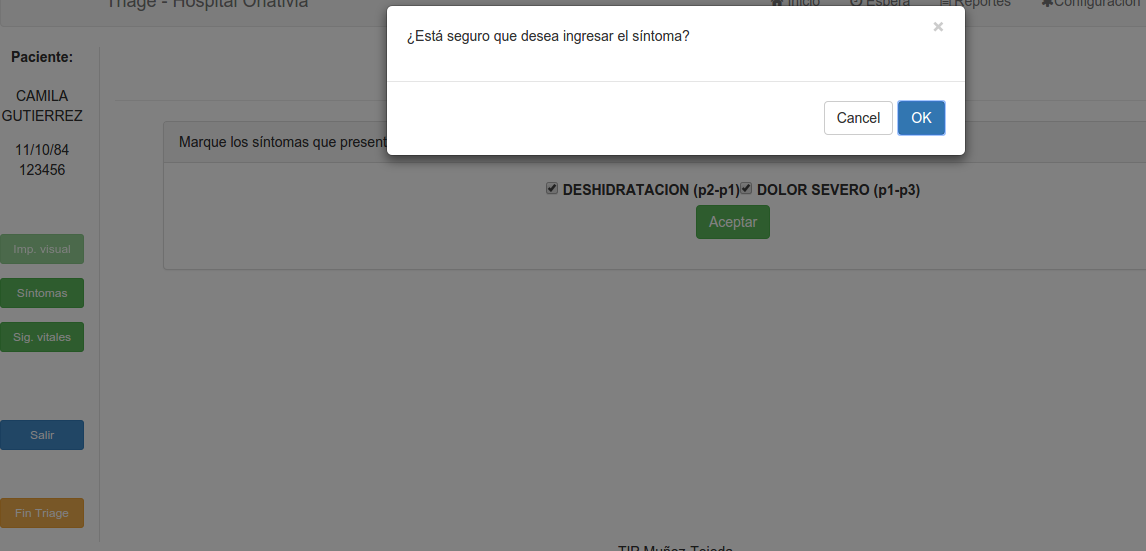
\includegraphics[width=0.99\textwidth]{impresion_visual_p1.png}}
\caption{Pantalla inicial de Triage} \label{fig:impresion_visual_p1}
\end{figure}
Si el usuario confirma, el sistema deriva directamente a la pantalla de Prioridad UNO, mostrando los datos y síntomas del paciente ingresado (figura \ref{fig:prioridad_uno}).
\begin{figure}
\centerline{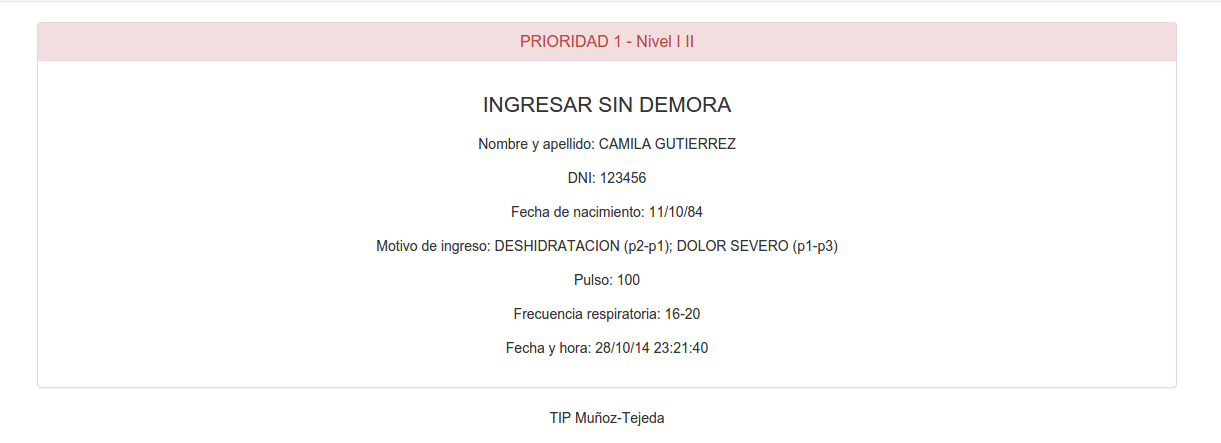
\includegraphics[width=0.99\textwidth]{prioridad_uno.png}}
\caption{Prioridad UNO} \label{fig:prioridad_uno}
\end{figure}

\subsection{Síntomas}
En la pestaña de síntomas (figura \ref{fig:sintomas})
\begin{figure}
\centerline{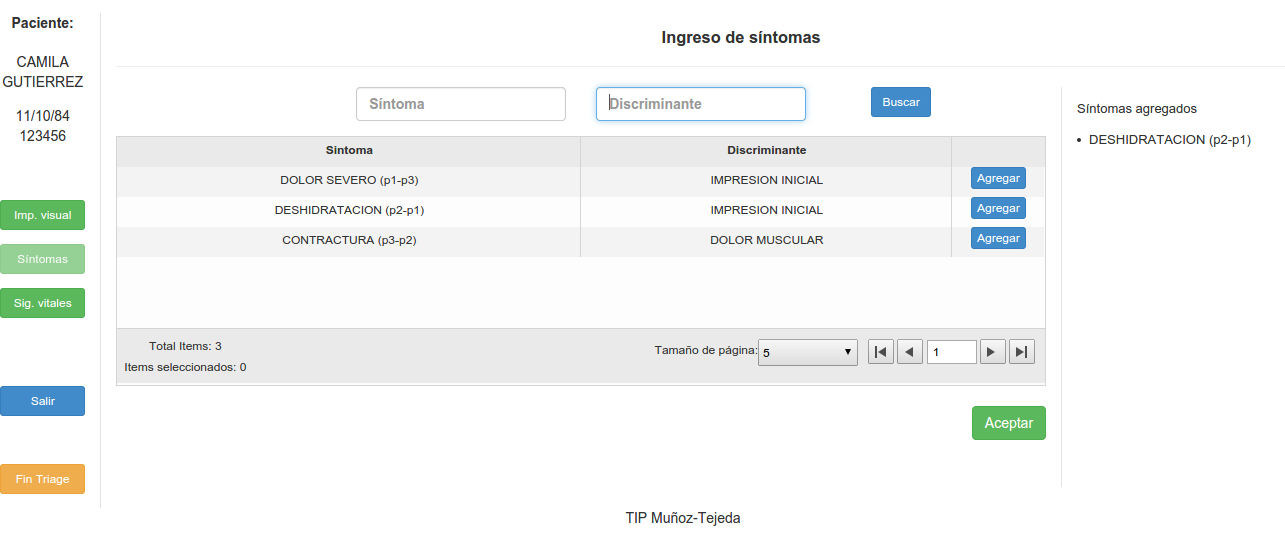
\includegraphics[width=0.99\textwidth]{sintomas.png}}
\caption{Pestaña de síntomas} \label{fig:sintomas}
\end{figure}
van a ser cargados los síntomas que el paciente informe. 

En el cuadro central se pueden ver todos los síntomas cargados en sistema, indicando cuál es su discriminante. Aquí se puede filtrar también por síntoma o discriminante (tal como se explica en la sección 'Filtrado del listado') (Ver figura \ref{fig:sintomas_filtrar}).
\begin{figure}
\centerline{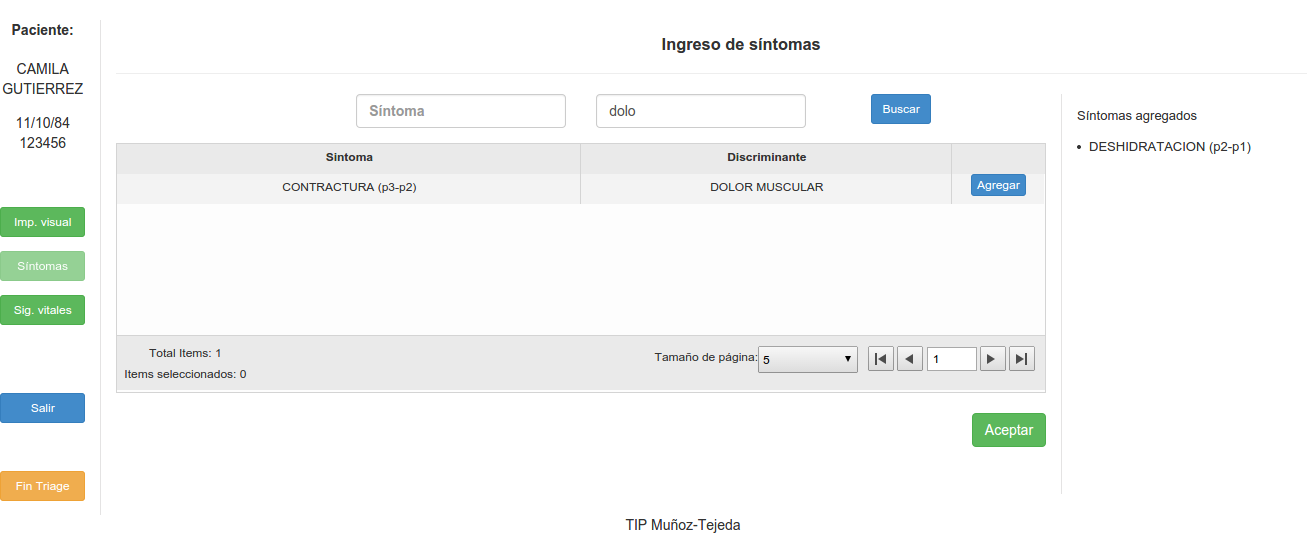
\includegraphics[width=0.99\textwidth]{sintomas_buscar.png}}
\caption{Filtrado en el cuadro de síntomas} \label{fig:sintomas_filtrar}
\end{figure}
Una vez filtrado el listado y encontrado lo que se busca, en cada fila del cuadro se puede ver el botón ``Agregar'' (figura \ref{fig:sintomas_agregar}), que permite cargar un nuevo síntoma al paciente.
\begin{figure}
\centerline{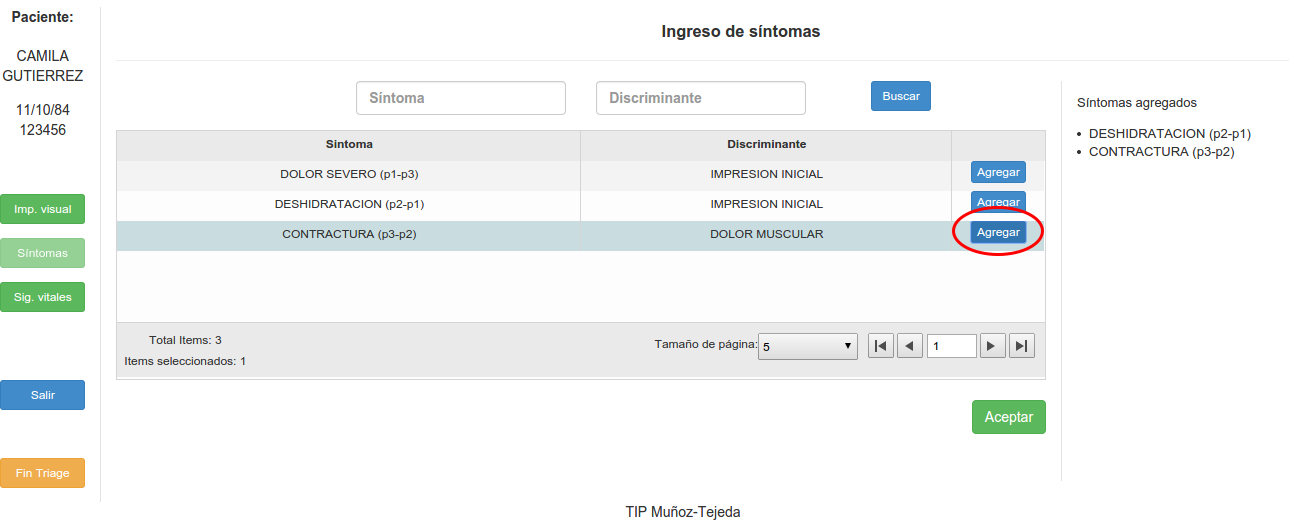
\includegraphics[width=0.99\textwidth]{sintomas_agregar.png}}
\caption{Agregar nuevo síntoma} \label{fig:sintomas_agregar}
\end{figure}
En la parte derecha de la pantalla se pueden ver los síntomas ya cargados. Se puede también eliminar algún síntoma agregado mediante el botón ``Borrar'' (que aparece al pararse con el puntero sobre el elemento a eliminar).

En el caso de ingresar un síntoma con Prioridad UNO,  el sistema corta la interacción con el usuario con un cartel de confirmación. Si el usuario confirma que efectivamente ese es el síntoma a agregar, el sistema deriva directamente a la pantalla de Prioridad UNO, mostrando los datos y síntomas del paciente ingresado (figura \ref{fig:prioridad_uno}).

Al finalizar con la carga, se debe presionar el botón ``Aceptar'' para grabar los síntomas seleccionados.


\subsection{Signos Vitales}
La tercer pestaña del Triage es para completar los signos vitales del paciente (figura \ref{fig:signos_vitales}).
\begin{figure}
\centerline{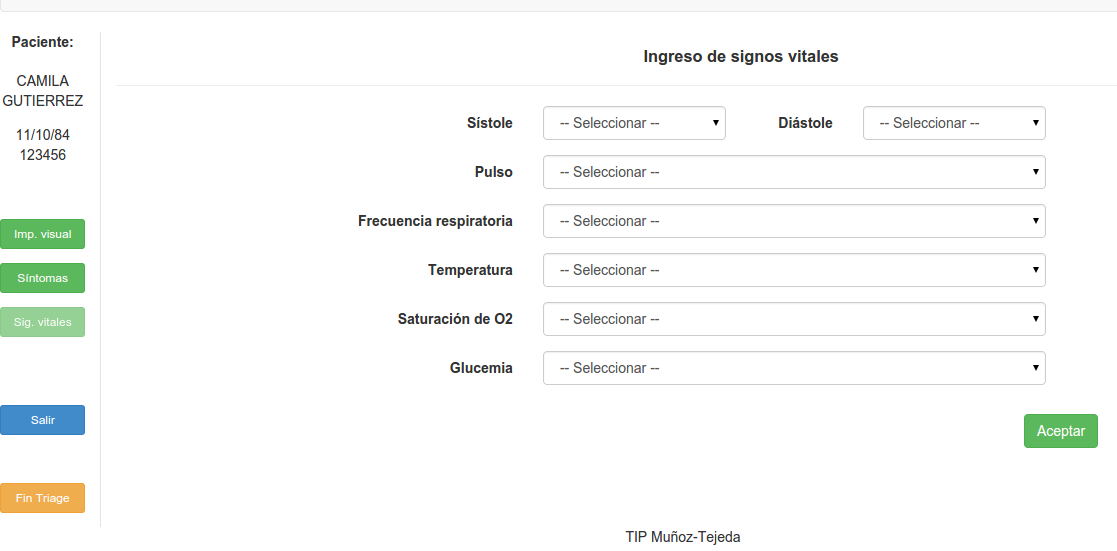
\includegraphics[width=0.99\textwidth]{signos_vitales.png}}
\caption{Signos Vitales} \label{fig:signos_vitales}
\end{figure}
Cada signo vital está definido para ser seleccionado de una lista acotada. En el caso de seleccionar algún valor que corresponda a una Prioridad UNO, el sistema mostrará un mensaje de confirmación. Si el usuario confirma la acción, se corta toda interacción mostrando la pantalla que indica atención inmediata (figura \ref{fig:prioridad_uno}).

Al finalizar de cargar los signos vitales, se debe presionar el botón ``Guardar'' (figura \ref{fig:signos_vitales_guardar})
\begin{figure}
\centerline{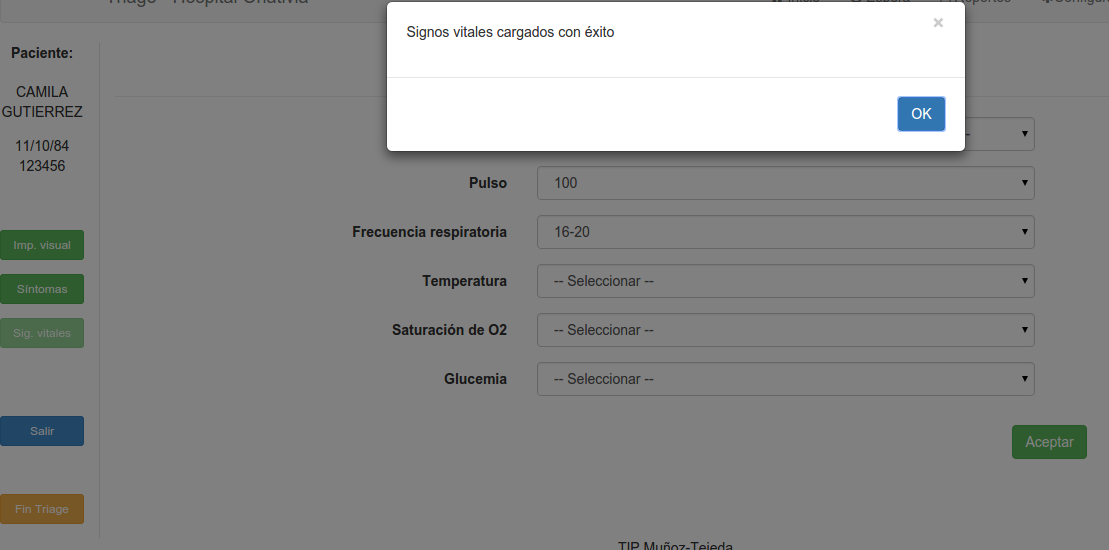
\includegraphics[width=0.99\textwidth]{signos_vitales_guardar.png}}
\caption{Signos Vitales} \label{fig:signos_vitales_guardar}
\end{figure}
y el sistema informará que los datos se han guardado con éxito.


\subsection{Fin de la carga}
Al terminar de cargar los síntomas hay dos caminos:
\begin{description}
\item[Finalizar Triage]  \mbox{} \\
Para finalizar el Triage, se debe presionar el botón sobre la pestaña izquieda llamado ``Fin Triage'' (figura \ref{fig:fin_triage}).
\begin{figure}
\centerline{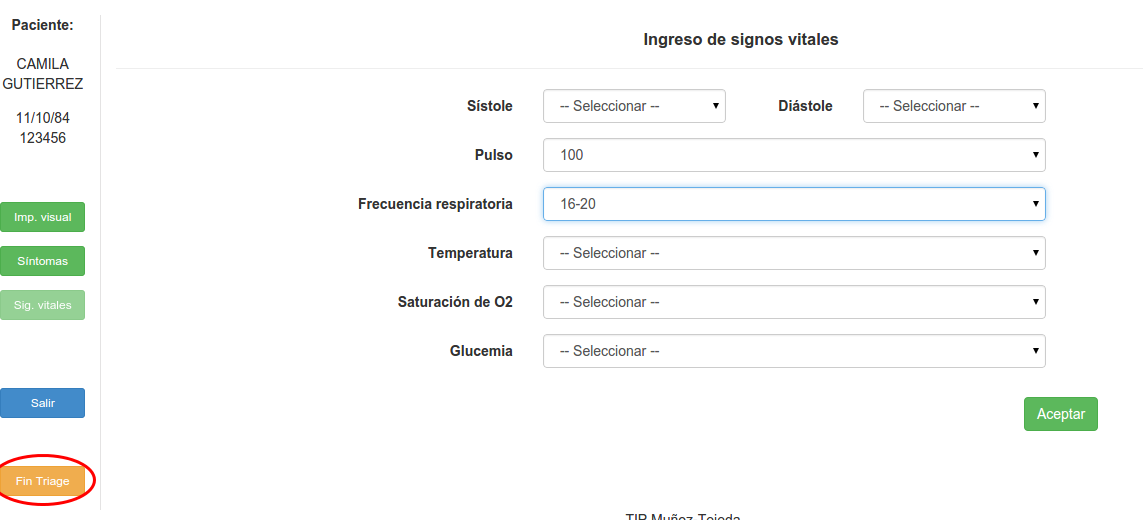
\includegraphics[width=0.99\textwidth]{fin_triage.png}}
\caption{Signos Vitales} \label{fig:fin_triage}
\end{figure}
 Al hacer esto, el sistema calcula la prioridad del paciente, indicando todos los síntomas cargados y sus datos personales. 

Esta acción sólo puede mostrar las pantallas de Prioridad DOS (figura \ref{fig:prioridad_dos}) 
\begin{figure}
\centerline{
\includegraphics[width=0.99\textwidth]{prioridad_dos.png}}
\caption{Prioridad DOS} \label{fig:prioridad_dos}
\end{figure}
y Prioridad TRES (figura \ref{fig:prioridad_tres}), 
\begin{figure}
\centerline{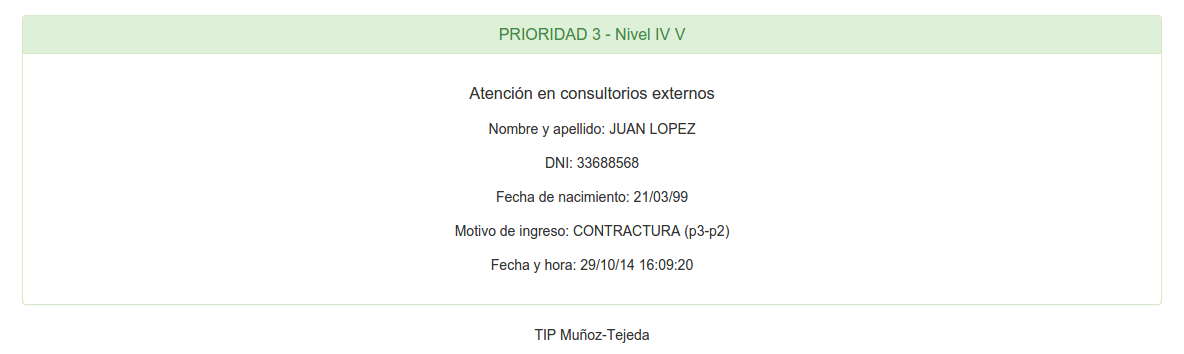
\includegraphics[width=0.99\textwidth]{prioridad_tres.png}}
\caption{Signos Vitales} \label{fig:prioridad_tres}
\end{figure}
ya que la pantalla de Prioridad UNO sólo se presenta al seleccionar un síntoma de Prioridad UNO y corta toda interacción con el usuario.
Finalizar el Triage no quita al paciente de la lista de espera, simplemente calcula su prioridad. 

\item[Salir de la carga]\mbox{} \\
En el caso de querer abandonar la carga de síntomas para poder retomarla más tarde, el sistema provee la acción ``Salir'' (figura \ref{fig:fin}),
\begin{figure}
\centerline{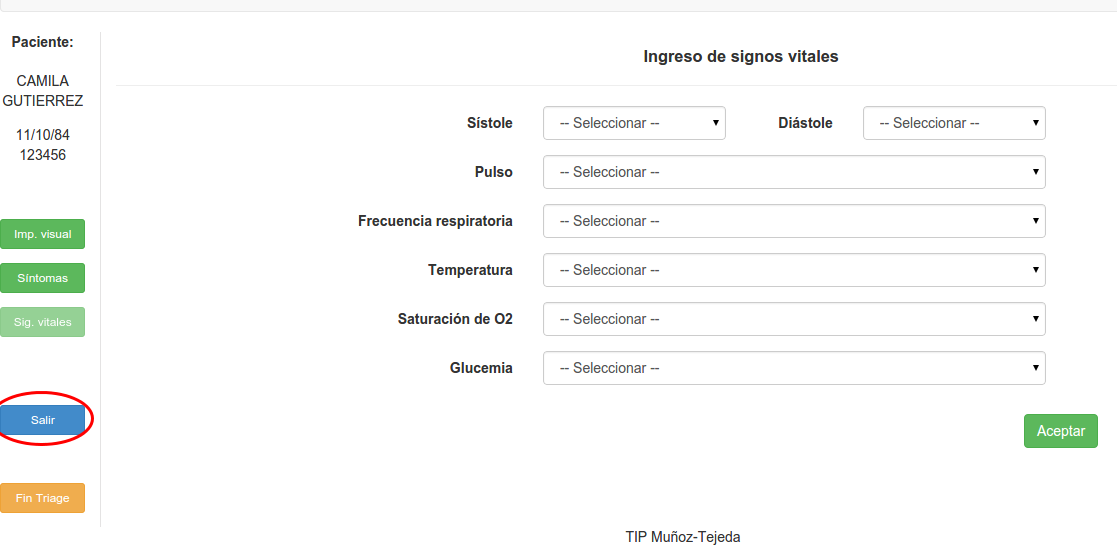
\includegraphics[width=0.99\textwidth]{fin.png}}
\caption{Signos Vitales} \label{fig:fin}
\end{figure}
que permite guardar los síntomas ingresados hasta el momento y poder recuperarlos si se carga el paciente desde la lista de espera.


\end{description}

\section{Pacientes en espera}
En la secciones anteriores se describió la manera de completar el Triage. 

Cada vez que se termina de cargar los síntomas hay dos caminos: ``Fin Triage'' o ``Salir''. Ambas opciones dejan al paciente en una ``Lista de espera'' (figura \ref{fig:espera}).
\begin{figure}
\centerline{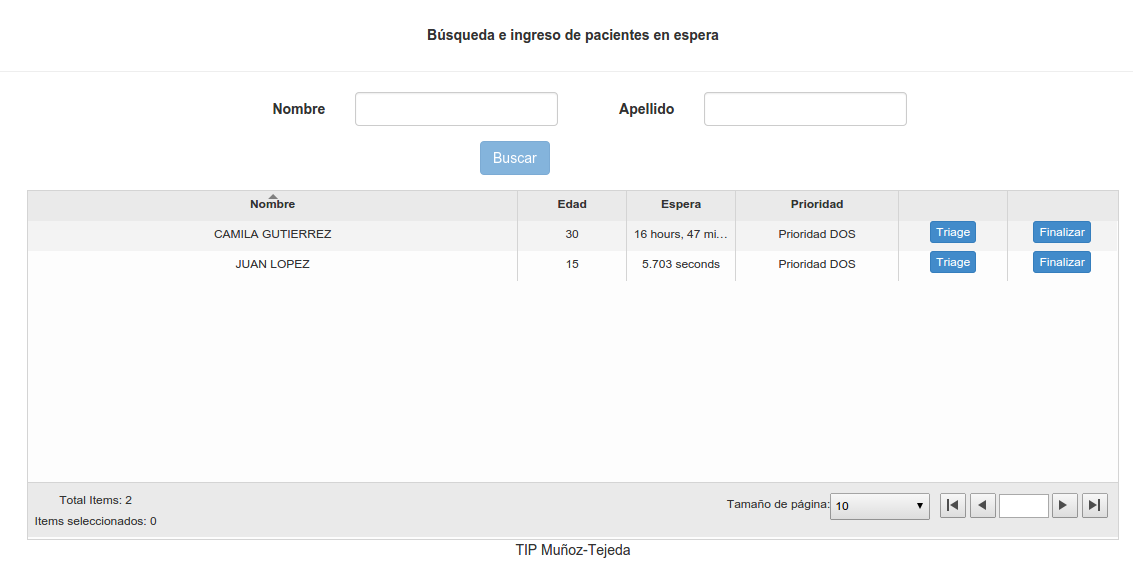
\includegraphics[width=0.99\textwidth]{espera.png}}
\caption{Signos Vitales} \label{fig:espera}
\end{figure}
 La pantalla de lista de espera contiene un cuadro como los vistos anteriormente para la búsqueda de personas así como los filtros para realizar búsquedas en ese cuadro.

Esta pantalla es muy útil cuando la carga de síntomas es realizada por dos personas en ubicaciones físicas distinas. El paciente puede ser atendido en un mostrador (donde se toman sus síntomas, por ejemplo), y luego pasar a un consultorio para la toma de signos vitales. El enfermero en el consultorio debe solamente buscar al paciente en la lista de espera y podrá continuar grabando sus síntomas sin perder ninguna información ya cargada.

\subsubsection{Continuar el Triage}
En el caso de querer continuar el Triage de un paciente en lista de espera, el sistema permite buscar al paciente utilizando el filtro. Una vez localizado, a nivel fila del cuadro encontramos la opción ``Triage'' (figura \ref{fig:espera1})
\begin{figure}
\centerline{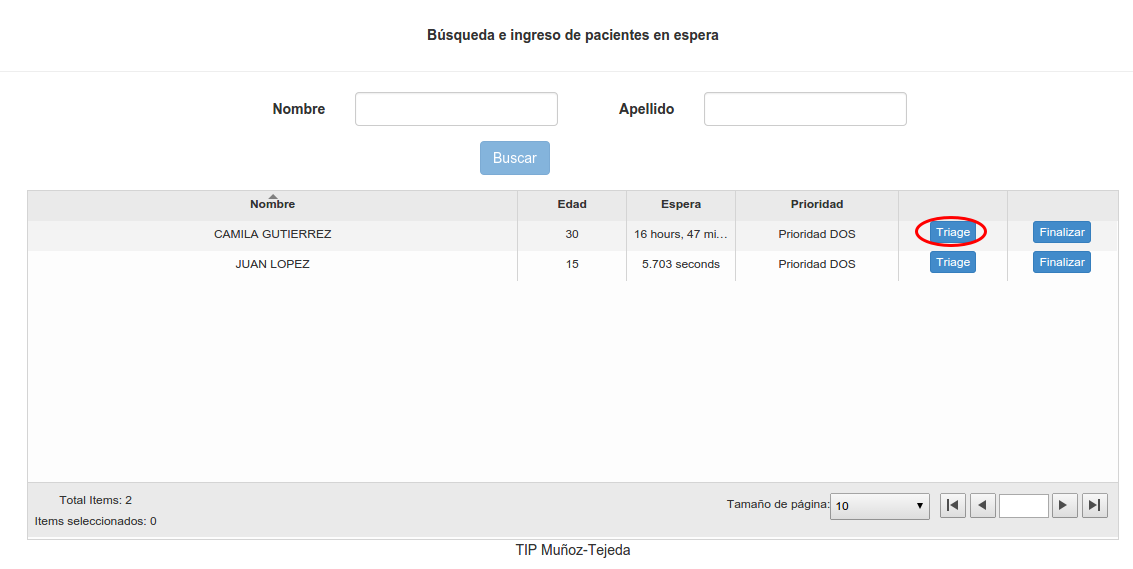
\includegraphics[width=0.99\textwidth]{espera1.png}}
\caption{Signos Vitales} \label{fig:espera1}
\end{figure}
que permite volver a la pantalla de Triage del paciente seleccionado para continuar cargando síntomas.


\mySection{Reportes}
En esta sección explicamos como generar los tres tipos de reportes que realiza el sistema: cantidad de consultas según prioridad, promedio de tiempos de espera según prioridad e historial de atenciones por paciente.

\mySubSection{Reporte de cantidad de consultas según prioridad}
Para acceder a la pantalla del reporte de cantidad de consultas según prioridad nos dirigimos hacia ``Reportes'' y luego a ``Prioridades'' (ver figura \ref{fig:menu_reporte_prioridades}).
\begin{figure}
\centerline{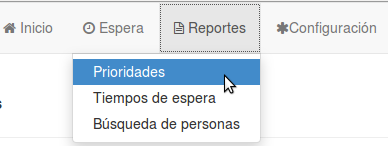
\includegraphics[width=0.7\textwidth]{menu_reporte_prioridades.png}}
\caption{Menú de reporte de prioridades}
\label{fig:menu_reporte_prioridades}
\end{figure}
Allí debemos ingresar la fecha inicial y la fecha final para delimitar las consultas a considerar dentro del reporte. Luego presionamos el botón ``Generar'' para obtener el reporte en pantalla (figura \ref{fig:reporte_prioridades}).
\begin{figure}
\centerline{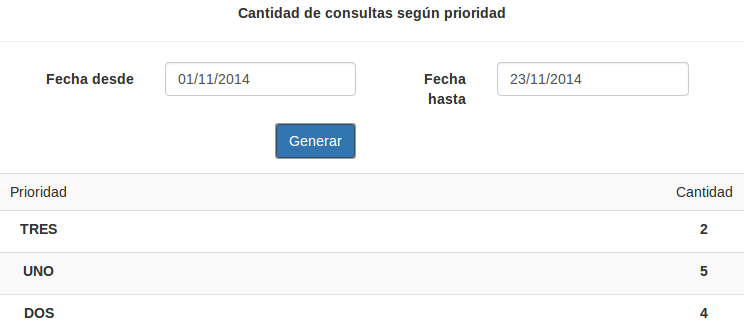
\includegraphics[width=1\textwidth]{reporte_prioridades.png}}
\caption{Reporte de cantidad de consultas según prioridad}
\label{fig:reporte_prioridades}
\end{figure}

\mySubSection{Reporte de promedio de tiempos de espera según prioridad}
Para acceder a la pantalla del reporte de promedio de tiempos de espera según prioridad nos dirigimos hacia ``Reportes'' y luego a ``Tiempos de espera'' (ver figura \ref{fig:menu_reporte_tiempos_espera}).
\begin{figure}
\centerline{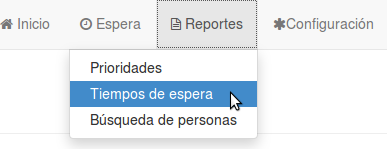
\includegraphics[width=0.7\textwidth]{menu_reporte_tiempos_espera.png}}
\caption{Menú de reporte de tiempos de espera}
\label{fig:menu_reporte_tiempos_espera}
\end{figure}
Allí, al igual que con el reporte de cantidad de consultas, debemos ingresar la fecha inicial y la fecha final para delimitar las atenciones a considerar dentro del reporte. Luego presionamos el botón ``Generar'' para obtener el reporte en pantalla (figura \ref{fig:reporte_tiempos_espera}).
\begin{figure}
\centerline{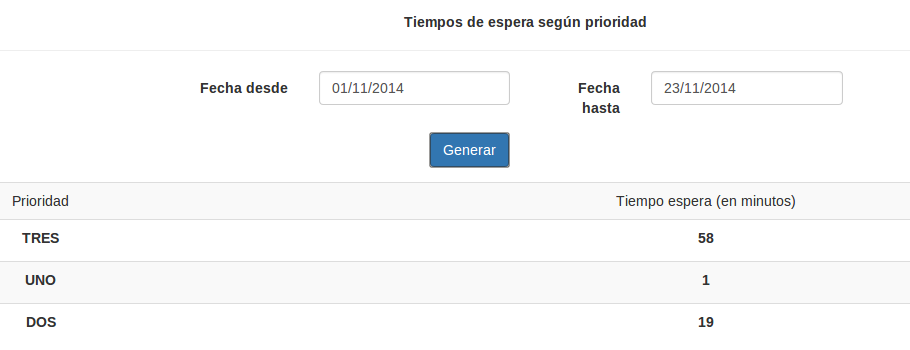
\includegraphics[width=1\textwidth]{reporte_tiempos_espera.png}}
\caption{Reporte de tiempos de espera según prioridad}
\label{fig:reporte_tiempos_espera}
\end{figure}

\mySubSection{Reporte de historial de atenciones por paciente}
Para acceder a la pantalla del reporte de historial de atenciones por paciente nos dirigimos hacia ``Reportes'' y luego a ``Búsqueda de personas'' (ver figura \ref{fig:menu_reporte_pacientes}).
\begin{figure}
\centerline{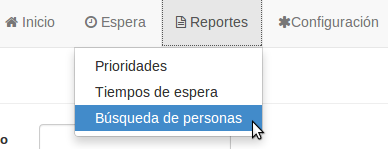
\includegraphics[width=0.7\textwidth]{menu_reporte_pacientes.png}}
\caption{Menú de reporte de historial de atenciones por paciente}
\label{fig:menu_reporte_pacientes}
\end{figure}
Allí podemos buscar el paciente que deseemos por DNI, apellido, fecha de nacimiento o nombre . Una vez encontrado el paciente presionamos el botón ``Detalle'' del listado (ver figura \ref{fig:listado_pacientes}) para ingresar en la pantalla del detalle de atenciones.
\begin{figure}
\centerline{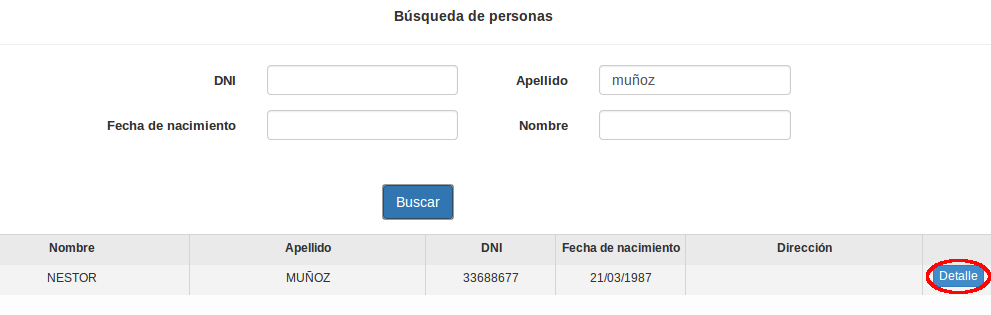
\includegraphics[width=1\textwidth]{listado_pacientes.png}}
\caption{Listado de pacientes}
\label{fig:listado_pacientes}
\end{figure}
Allí se nos muestran los datos personales del paciente más un listado con todas las atenciones que recibió (figura \ref{fig:historial_paciente}).
\begin{figure}
\centerline{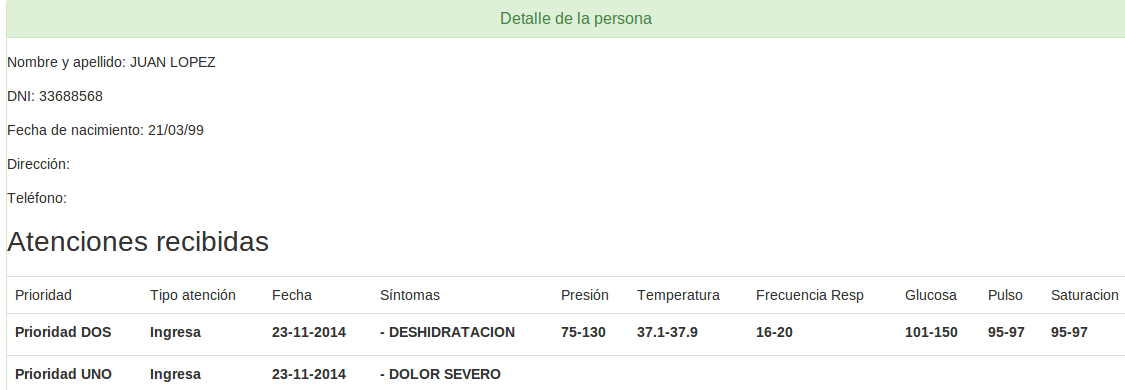
\includegraphics[width=1\textwidth]{historial_paciente.png}}
\caption{Historial de atenciones del paciente}
\label{fig:historial_paciente}
\end{figure}

\mySection{Alta, baja y modificación (ABM) de datos del sistema}
En esta sección explicamos como realizar el alta, baja y modificación de datos del sistema, es decir, síntomas, discriminantes y usuarios.

\mySubSection{Acceso al menú de configuración}
Para acceder al menú de configuración de datos, el usuario actual debe tener el rol de administrador (explicaremos la asignación de roles en la sección \ref{ABM_usuarios}). En caso contrario dicho menú permanecerá oculto (ver figuras \ref{fig:menu_conf_visible} y \ref{fig:menu_conf_oculto}).

\begin{figure}
\centerline{
\includegraphics[width=0.7\textwidth]{menu_configuracion_visible.png}}
\caption{Menú de configuración visible}
\label{fig:menu_conf_visible}
\end{figure}

\begin{figure}
\centerline{
\includegraphics[width=0.7\textwidth]{menu_configuracion_oculto.png}}
\caption{Menú de configuración oculto}
\label{fig:menu_conf_oculto}
\end{figure}

\mySubSection{ABM de síntomas}\label{cap:ABM_sintomas}
Para acceder a la pantalla de administración de síntomas nos dirigimos hacia ``Configuración'' y luego a ``Síntomas'' (ver figura \ref{fig:menu_sintomas}).
\begin{figure}
\centerline{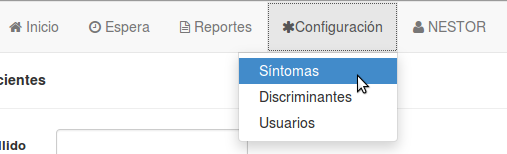
\includegraphics[width=0.7\textwidth]{menu_sintomas.png}}
\caption{Menú de síntomas}
\label{fig:menu_sintomas}
\end{figure}
Allí se nos muestra el listado de todos los síntomas cargados en el sistema (figura \ref{fig:listado_sintomas}).

\begin{figure}
\centerline{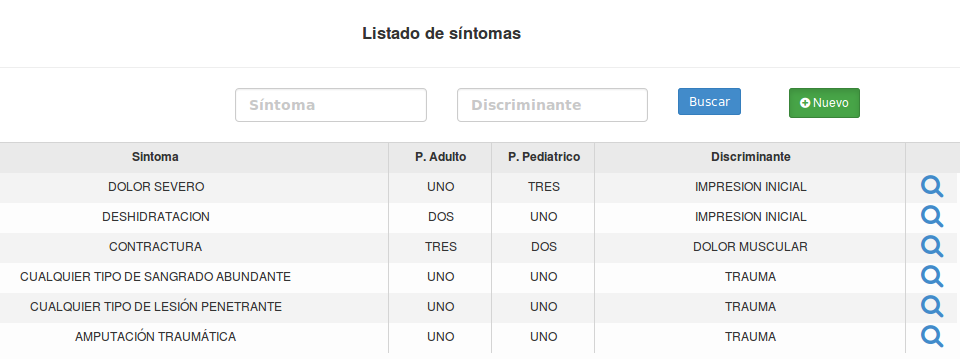
\includegraphics[width=1\textwidth]{listado_sintomas.png}}
\caption{Listado de síntomas}
\label{fig:listado_sintomas}
\end{figure}

\begin{description}
\item[Alta de síntoma] \mbox{} \\
%\subsubsection{Alta de síntoma}\label{cap:alta_sintoma}
En la pantalla del listado de síntomas hacemos click en el botón ``Nuevo'' que nos dirige a la pantalla del detalle del síntoma (figura \ref{fig:detalle_sintoma}).
\begin{figure}
\centerline{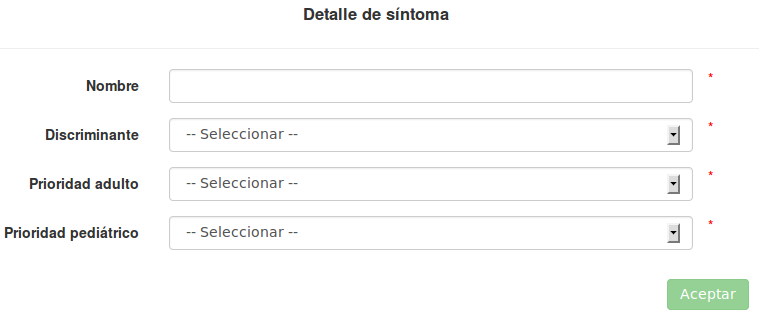
\includegraphics[width=1\textwidth]{detalle_sintoma.png}}
\caption{Detalle de síntoma}
\label{fig:detalle_sintoma}
\end{figure}
Allí debemos ingresar el nombre, el discriminante, la prioridad para adultos y la prioridad para pediátricos. Tener en cuenta que si el discriminante que deseamos no aparece en el listado desplegable entonces primero debemos darle de alta (ver sección \ref{cap:ABM_discriminantes}). Luego de llenar todos los campos, el botón ``Aceptar'' se desbloquea y si le hacemos click debería aparecer un mensaje que confirma que el síntoma fue ingresado con éxito.

\item[Modificación de síntoma] \mbox{} \\
%\subsubsection{Modificación de síntoma}\label{cap:modificacion_sintoma}
Para modificar un síntoma debemos seleccionarlo del listado. Para facilitar la búsqueda del mismo podemos filtrar el listado llenando los campos de ``Síntoma'' y/o ``Discriminante'' (ver sección \ref{cap:filtrado_listado}). Si encontramos el registro buscado hacemos click en el botón ``Ver detalle''(ver figura \ref{fig:sintomas_filtro}) 
\begin{figure}
\centerline{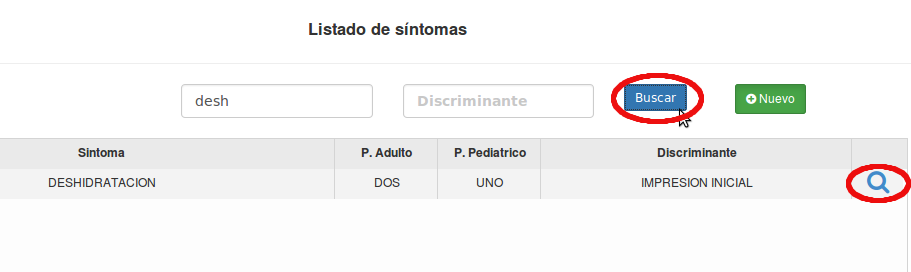
\includegraphics[width=1\textwidth]{sintomas_listado_buscar.png}}
\caption{Listado de síntomas filtrado. Aparecen los botones ``Buscar'' y ``Ver detalle'' señalados en rojo}
\label{fig:sintomas_filtro}
\end{figure}
que nos lleva a la pantalla de ``Detalle de síntoma'' con todos los campos cargados. Allí podemos modificar los valores que deseemos y al presionar el botón ``Aceptar'' debería aparecer el mensaje de confirmación de síntoma actualizado con éxito.

\item[Baja de síntoma] \mbox{} \\
%\subsubsection{Baja de síntoma}
Una vez creados, los síntomas no se pueden eliminar. Solo se pueden modificar como explicamos en la sección anterior. Lo mismo sucede con los discriminantes.

\end{description}

\mySubSection{ABM de discriminantes de síntomas}\label{cap:ABM_discriminantes}
Para acceder a la pantalla de administración de discriminantes nos dirigimos hacia ``Configuración'' y luego a ``Discriminantes'' (ver figura \ref{fig:menu_discriminantes}).
\begin{figure}
\centerline{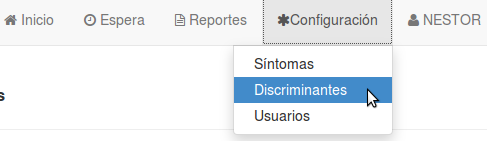
\includegraphics[width=0.7\textwidth]{menu_discriminantes.png}}
\caption{Menú de discriminantes de síntomas}
\label{fig:menu_discriminantes}
\end{figure}
Allí se nos muestra el listado de todos los discriminantes cargados en el sistema (figura \ref{fig:listado_discriminantes}).
\begin{figure}
\centerline{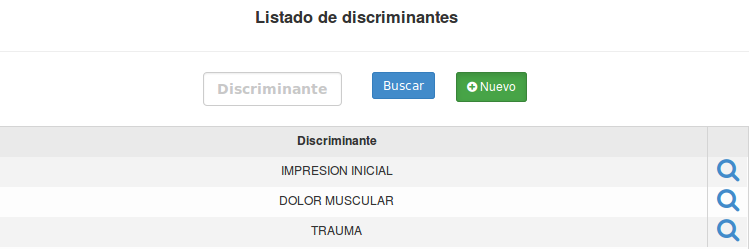
\includegraphics[width=1\textwidth]{listado_discriminantes.png}}
\caption{Listado de discriminantes de síntomas}
\label{fig:listado_discriminantes}
\end{figure}

\begin{description}
\item[Alta de discriminante de síntoma] \mbox{} \\
%\subsubsection{Alta de discriminante de síntoma}\label{cap:alta_discriminante}
En la pantalla del listado de discriminantes hacemos click en el botón ``Nuevo'' que nos dirige a la pantalla del detalle del discriminante (figura \ref{fig:nuevo_discriminante}).
\begin{figure}
\centerline{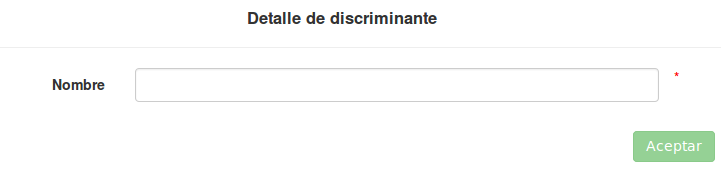
\includegraphics[width=1\textwidth]{nuevo_discriminante.png}}
\caption{Alta de discriminante de síntoma}
\label{fig:nuevo_discriminante}
\end{figure}
Allí debemos ingresar el nombre, lo que desbloquea el botón ``Aceptar'' y si le hacemos click debería aparecer un mensaje que confirma que el discriminante fue ingresado con éxito. Una vez cargado podremos ingresar nuevos síntomas de ese discriminante, como explicamos anteriormente en la sección \ref{cap:ABM_sintomas}.

\item[Modificación de un discriminante de síntoma] \mbox{} \\
%\subsubsection{Modificación de un discriminante de síntoma}
Para modificar el nombre de un discriminante debemos seleccionarlo del listado\footnote{Por cuestiones de lógica del proceso de Triage podemos modificar el nombre de cualquier discriminante a excepción de ``IMPRESIÓN INICIAL''.}. Para facilitar la búsqueda del mismo podemos filtrar el listado llenando el campo ``Discriminante'' (ver sección \ref{cap:filtrado_listado}). Si encontramos el registro buscado hacemos click en el botón ``Ver detalle'' que nos lleva a la pantalla de ``Detalle de discriminante'' con el campo ``Nombre'' cargado y con un listado que nos muestra todos los síntomas de ese discriminante (ver figura \ref{fig:detalle_discriminante}).
\begin{figure}
\centerline{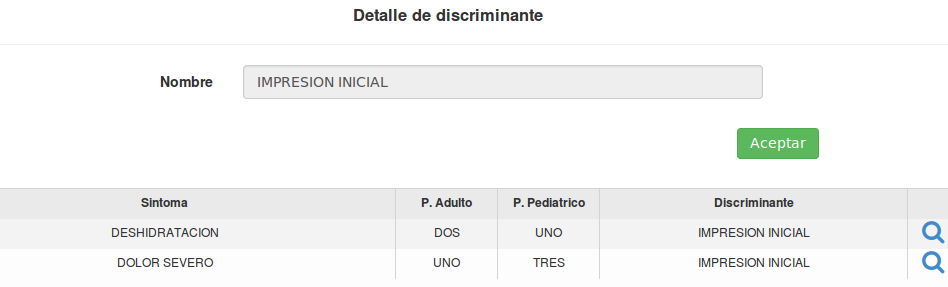
\includegraphics[width=1\textwidth]{listado_sintomas_de_discriminante.png}}
\caption{Detalle del discriminante con listado de síntomas}
\label{fig:detalle_discriminante}
\end{figure}
En esa pantalla podemos modificar el nombre y al presionar el botón ``Aceptar'' debería aparecer el mensaje de confirmación de discriminante actualizado con éxito. También podemos hacer click en el botón ``Ver detalle'' de algún síntoma del listado para ir a la pantalla de ``Detalle de síntoma'' y modificarlo como mostramos anteriormente en la sección \ref{cap:ABM_sintomas}.

\item[Baja de discriminante de síntoma] \mbox{} \\
%\subsubsection{Baja de discriminante de síntoma}
Al igual que los síntomas, una vez creados, los discriminantes no se pueden eliminar. Solo podemos modificarles el nombre como explicamos en la sección anterior.
\end{description}

\mySubSection{ABM de usuarios}\label{ABM_usuarios}
Para acceder a la pantalla de administración de usuarios nos dirigimos hacia ``Configuración'' y luego a ``Usuarios'' (ver figura \ref{fig:menu_usuarios}).
\begin{figure}
\centerline{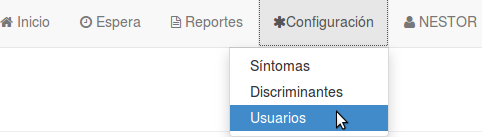
\includegraphics[width=0.7\textwidth]{menu_usuarios.png}}
\caption{Menú de usuarios}
\label{fig:menu_usuarios}
\end{figure}
Allí se nos muestra el listado de todos los usuarios cargados en el sistema (figura \ref{fig:listado_usuarios}).
\begin{figure}
\centerline{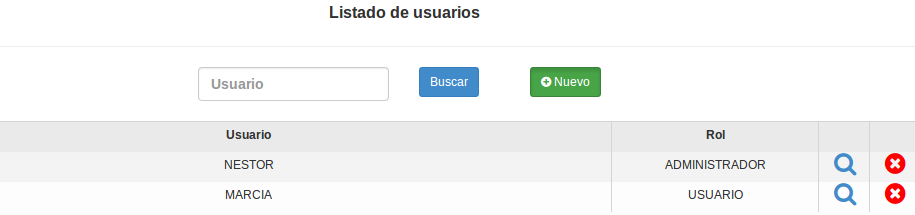
\includegraphics[width=1\textwidth]{listado_usuarios.png}}
\caption{Listado de usuarios}
\label{fig:listado_usuarios}
\end{figure}

\begin{description}
\item[Roles] \mbox{} \\
%\subsubsection{Roles}\label{cap:roles}
Hay dos roles: ``administrador'' y ``usuario''. El usuario con rol ``administrador'' puede ingresar en todas las pantallas de la aplicación. En cambio, el usuario con rol ``usuario'' puede ingresar en todas las pantallas excepto en la de configuración.

\item[Alta de usuario] \mbox{} \\
%\subsubsection{Alta de usuario}\label{cap:alta_usuario}
En la pantalla del listado de usuarios hacemos click en el botón ``Nuevo'' que nos dirige a la pantalla del detalle del usuario (figura \ref{fig:nuevo_usuario}).
\begin{figure}
\centerline{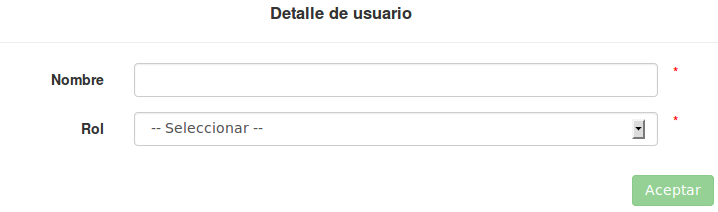
\includegraphics[width=1\textwidth]{nuevo_usuario.png}}
\caption{Alta de usuario}
\label{fig:nuevo_usuario}
\end{figure}
Allí ingresamos el nombre y el rol, y luego presionamos el botón ``Aceptar'' (que desbloqueamos al llenar todos los campos). Nos debería aparecer un mensaje que confirma que el usuario fue ingresado con éxito. Una vez cargado podremos ingresar a la aplicación con ese usuario. Tener en cuenta que todos los usuarios son creados con la contraseña ``triage" (anteriormente explicamos cómo cambiarla en la sección \ref{cap:cambio_pass}).

\item[Modificación de usuario] \mbox{} \\
%\subsubsection{Modificación de un usuario}
Para modificar el nombre o el rol de un usuario debemos seleccionarlo del listado. Para facilitar la búsqueda del mismo podemos filtrar el listado llenando el campo ``Usuario'' (ver sección \ref{cap:filtrado_listado}). Si encontramos el registro buscado hacemos click en el botón ``Ver detalle'' que nos lleva a la pantalla de ``Detalle de usuario'' con todos los campos cargados. Allí podemos modificar los valores que deseemos y al presionar el botón ``Aceptar'' debería aparecer el mensaje de confirmación de usuario actualizado con éxito. Tener en cuenta que el usuario modificado será deslogueado.

\item[Baja de usuario] \mbox{} \\
Para dar de baja un usuario debemos presionar el botón ``Eliminar'' del listado. Si confirmamos la acción deberia aparecer el mensaje de ``Usuario eliminado con éxito'' (figura \ref{fig:eliminar_usuario}).
\begin{figure}
\centerline{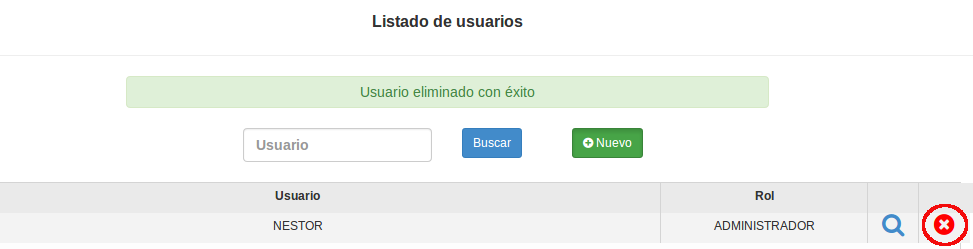
\includegraphics[width=1\textwidth]{eliminar_usuario.png}}
\caption{Baja de usuario}
\label{fig:eliminar_usuario}
\end{figure}
El usuario será deslogueado y ya no podrá ingresar a la aplicación. Tener en cuenta que el sistema no permite que se eliminen todos los usuarios administradores.

\end{description}

\end{document}